\documentclass{ansarticle-preprint}
%\usepackage{ucs}
\usepackage[utf8]{inputenc}
\usepackage{amsmath}
%\usepackage{cite}
\usepackage{anslistings}
\usepackage{multicol}
\usepackage{pdfsync}
\usepackage{enumitem}

\usepackage{pgfplots}
\usepackage{pgfplotstable}

\usepackage{fontenc}
\usepackage{graphicx}
\usepackage{xspace}

\usepackage{siunitx}

\usepackage{floatflt}

\usepackage{multirow}

%\renewcommand{\baselinestretch}{2.0}

\graphicspath{{svg/}}

\usepackage[normalem]{ulem}

\usepackage{caption}
\usepackage{subcaption}

\usepackage{todonotes}

\pgfplotsset{compat=1.9}
\definecolor{gnuplot@lightblue}{RGB}{87,181,232}
\definecolor{gnuplot@green}{RGB}{0,158,115}
\definecolor{gnuplot@purple}{RGB}{148,0,212}

\newcommand{\specialword}[1]{\texttt{#1}}
\newcommand{\dealii}{{\specialword{deal.II}}\xspace}
\newcommand{\pfrst}{{\specialword{p4est}}\xspace}
\newcommand{\trilinos}{{\specialword{Trilinos}}\xspace}
\newcommand{\aspect}{\specialword{Aspect}\xspace}
\newcommand{\petsc}{\specialword{PETSc}\xspace}
\newcommand{\cmake}{{\specialword{CMake}}\xspace}
\newcommand{\candi}{{\specialword{candi}}\xspace}



\usetikzlibrary{shapes.misc}
\tikzset{cross/.style={cross out, draw=black, minimum size=2*(#1-\pgflinewidth), inner sep=0pt, outer sep=0pt},
%default radius will be 1pt.
cross/.default={2pt}}

%
% Author list -- please add yourself in both places below (in
%                alphabetical order) if you think that your
%                contributions to the last release warrant this
%

\hypersetup{
  pdfauthor={
    Daniel Arndt,
    Wolfgang Bangerth,
    Marco Feder,
    Marc Fehling,
    Rene Gassm\"{o}ller,
    Timo Heister,
    Luca Heltai,
    Martin Kronbichler,
    Matthias Maier,
    Peter Munch,
    Jean-Paul Pelteret,
    Simon Sticko,
    Bruno Turcksin,
    David Wells
  },
  pdftitle={The deal.II Library, Version 9.4, 2022},
}

\title{The \dealii Library, Version 9.4}

 \author[1*]{Daniel Arndt}
 \affil[1]{Scalable Algorithms and Coupled Physics Group,
   Computational Sciences and Engineering Division,
   Oak Ridge National Laboratory, 1 Bethel Valley Rd.,
   TN 37831, USA.
   \texttt{arndtd/turcksinbr@ornl.gov}}

 \author[2,3]{Wolfgang~Bangerth}
 \affil[2]{Department of Mathematics, Colorado State University, Fort
   Collins, CO 80523-1874, USA.
   \texttt{bangerth/marc.fehling@colostate.edu}}
 \affil[3]{Department of Geosciences, Colorado State University, Fort
   Collins, CO 80523, USA.}

   \author[4]{Marco~Feder}
\affil[4]{SISSA,
   International School for Advanced Studies,
   Via Bonomea 265,
   34136, Trieste, Italy.
   {\texttt{marco.feder/luca.heltai@sissa.it}}}

\author[2]{Marc~Fehling}

\author[5]{Rene~Gassm{\"o}ller}
\affil[5]{Department of Geological Sciences,
   University of Florida,
   1843 Stadium Road,
   Gainesville, FL, 32611, USA.
  {\texttt{rene.gassmoeller@ufl.edu}}}

\author[6]{Timo~Heister}
 \affil[6]{School of Mathematical and Statistical Sciences,
   Clemson University,
   Clemson, SC, 29634, USA
   {\texttt{heister@clemson.edu}}}

\author[4]{Luca~Heltai}

 \author[7,8]{Martin~Kronbichler}
 \affil[7]{Department of Information Technology,
   Uppsala University,
   Box 337, 751\,05 Uppsala, Sweden.
   {\texttt{martin.kronbichler/simon.sticko@it.uu.se}}}
 \affil[8]{Institute of Mathematics,
   University of Augsburg,
   Universit\"atsstr.~12a, 86159 Augsburg, Germany.
   {\texttt{martin.kronbichler@uni-a.de}}}

\author[9]{Matthias~Maier}
\affil[9]{Department of Mathematics,
  Texas A\&M University,
  3368 TAMU,
  College Station, TX 77845, USA.
  {\texttt{maier@math.tamu.edu}}}

\author[8,10]{Peter Munch}
 \affil[10]{Institute of Material Systems Modeling,
 Helmholtz-Zentrum Hereon,
 Max-Planck-Str. 1, 21502 Geesthacht, Germany.
   {\texttt{peter.muench@hereon.de}}}


\author[11]{Jean-Paul~Pelteret}
\affil[11]{Independent researcher.
{\texttt{jppelteret@gmail.com}}}

\author[7,12]{Simon~Sticko}
\affil[12]{Department of Mathematics and Mathematical Statistics,
   Umeå University,
   SE-90187 Umeå, Sweden}

\author[1*]{Bruno~Turcksin}

\author[13]{David Wells}
\affil[13]{Department of Mathematics, University of North Carolina,
  Chapel Hill, NC 27516, USA.
  {\texttt{drwells@email.unc.edu}}}

\renewcommand{\labelitemi}{--}


\begin{document}
\maketitle

\footnotetext{%
  $^\ast$ This manuscript has been authored by UT-Battelle, LLC under Contract No.
  DE-AC05-00OR22725 with the U.S. Department of Energy.
  %The United States
  %Government retains and the publisher, by accepting the article for
  %publication, acknowledges that the United States Government retains a
  %non-exclusive, paid-up, irrevocable, worldwide license to publish or reproduce
  %the published form of this manuscript, or allow others to do so, for United
  %States Government purposes. The Department of Energy will provide public
  %access to these results of federally sponsored research in accordance with the
  %DOE Public Access Plan (http://energy.gov/downloads/doe-public-access-plan).
}


\begin{abstract}
  This paper provides an overview of the new features of the finite element
  library \dealii, version 9.4.
\end{abstract}



%%%%%%%%%%%%%%%%%%%%%%%%%%%%%%%%%%%%%%%%%%%%%%%%%%%%%%%%%%%%%%%%%%%%%%%%%%%%%%%%
%%%%%%%%%%%%%%%%%%%%%%%%%%%%%%%%%%%%%%%%%%%%%%%%%%%%%%%%%%%%%%%%%%%%%%%%%%%%%%%%
%%%%%%%%%%%%%%%%%%%%%%%%%%%%%%%%%%%%%%%%%%%%%%%%%%%%%%%%%%%%%%%%%%%%%%%%%%%%%%%%
\section{Overview}

\dealii version 9.4.0 was released June 10, 2022.
\todo{Update release date.}
This paper provides an
overview of the new features of this release and serves as a citable
reference for the \dealii software library version 9.4. \dealii is an
object-oriented finite element library used around the world in the
development of finite element solvers. It is available for free under the
GNU Lesser General Public License (LGPL). Downloads are available at
\url{https://www.dealii.org/} and \url{https://github.com/dealii/dealii}.

The major changes of this release are:
%
\begin{itemize}
  \item Advances in simplex- and mixed-mesh support (see Section~\ref{sec:simplex});
  \item Repartitioning of distributed meshes (see Section~\ref{sec:repartitioning});
  \item Advances in matrix-free infrastructure (see Section~\ref{sec:mf});
  \item Advances in multigrid infrastructure (see Section~\ref{sec:multigrid});
  \item CutFEM support (see Section~\ref{sec:cut});
  \item Experimental integration of the Computational Geometry Algorithms Library (CGAL) (see Section~\ref{sec:cgalwrappers});
  \item Performance improvements in the particle infrastructure (see Section~\ref{sec:particles});
  \item Improvements to unstructured communication (see Section~\ref{sec:CA});
  \item Three new tutorial programs and one new code gallery program (see Section~\ref{subsec:steps}).
\end{itemize}
%

While all of these major changes are discussed in detail in
Section~\ref{sec:major}, there
are a number of other noteworthy changes in the current \dealii release,
which we briefly outline in the remainder of this section:
%
\begin{itemize}
%  \item \texttt{AffineConstraints::make\_consistent\_in\_parallel()} allows
%  to make constraints consistent in parallel.
  \item The \texttt{DataOutResample} class interpolates values defined on one
  triangulation onto a second potentially unrelated triangulation.
  By using this class, one can output the result obtained on an
  unstructured mesh on a structured one (which might facilitate a more
  memory-efficient storage format, for example if this second
  triangulation is a uniformly refined rectangle or box), or one can create a slice in 3D.
  \item The new member function \texttt{find\_point\_owner\_rank()} of
        \texttt{parallel\allowbreak ::distributed::\allowbreak Tri\allowbreak angulation} allows one to find the MPI
  ranks of cells containing specified points.
  It is communication-free and leverages the functionality of \pfrst (>v.2.2).
  Its algorithm is described in \cite{burstedde2020parallel}. This information will
  enable efficient construction of the
  communication pattern used in the class \texttt{Utilties::\allowbreak MPI::\allowbreak RemotePointEvaluation}. Furthermore, this function could be used in the future to allow
  particle simulations in which particle movement is not
  limited by CFL conditions, as done in \cite{mirzadeh2016parallel}.
  \item The new function
  \texttt{GridGenerator::pipe\_junction()}
  generates a triangulation of three cone-shaped pipes that cross at a bifurcation point in any possible configuration.
  A manifold description is applied to the boundary, which can be extended into the volume via transfinite interpolation \cite{Gordon82} using the \texttt{TransfiniteInterpolationManifold} class \cite{dealII90}.
  \item A new DoF renumbering function \texttt{DoFRenumbering::support\_point\_wise()} which groups together
  shape functions by their support point. This functionality is useful in both developing nodal schemes since, e.g., the $x$, $y$, and $z$
  velocities at a point will be consecutive in the solution vector. It also improves interoperability with external libraries which expect
  data in this format.
  \item A new module \texttt{Utilities::MPI::LargeCount} which enables sending and receiving MPI messages containing more than $2^{31}$ objects.
  This library either uses the new MPI-4 functions, such as \texttt{MPI\_Send\_c()}, or an internal implementation of large objects for
  compatibility with MPI-3.
  \item The \texttt{FEInterfaceValues} class, which computes common quantities at the interface of two cells, has been overhauled to make it
  more consistent with the rest of the library and use more intuitive names for functions. For example,
  \texttt{FEInterfaceValues::jump\_gradient()} is now \texttt{FEInterfaceValues::jump\_in\_shape\_gradients()}. Several new
  functions, such as \texttt{FEInterfaceValues::get\_jump\_in\_function\_values()}, have also been added.
  \item Vectors attached to \texttt{DataOut} do not need to be in ghosted state anymore. Internally, we create a copy of the vector with appropriate ghosting.
\end{itemize}
%
The changelog lists more than 100 other features and bugfixes.




%%%%%%%%%%%%%%%%%%%%%%%%%%%%%%%%%%%%%%%%%%%%%%%%%%%%%%%%%%%%%%%%%%%%%%%%%%%%%%%%
%%%%%%%%%%%%%%%%%%%%%%%%%%%%%%%%%%%%%%%%%%%%%%%%%%%%%%%%%%%%%%%%%%%%%%%%%%%%%%%%
%%%%%%%%%%%%%%%%%%%%%%%%%%%%%%%%%%%%%%%%%%%%%%%%%%%%%%%%%%%%%%%%%%%%%%%%%%%%%%%%
\section{Major changes to the library}
\label{sec:major}

This release of \dealii contains a number of large and significant changes,
which will be discussed in this section.
It of course also includes a
vast number of smaller changes and added functionality; the details of these
can be found
\href{https://dealii.org/developer/doxygen/deal.II/changes_between_9_3_0_and_9_4_0.html}
{in the file that lists all changes for this release}; see \cite{changes94}.

%\newpage

%%%%%%%%%%%%%%%%%%%%%%%%%%%%%%%%%%%%%%%%%%%%%%%%%%%%%%%%%%%%%%%%%%%%%%%%%%%%%%%%
\subsection{Advances in simplex- and mixed-mesh support}\label{sec:simplex}

\dealii has supported simplex and mixed meshes since the previous
release, 9.3, on an experimental basis.
We have continued to work on this support; the current state is
sufficient to support several larger-scale programs, although not all
functionality in \dealii works with such meshes yet. Specifically,
we have fixed many bugs and generalized existing functions that
previously only worked for hypercube-shaped cells. The most notable
new functionalities are:

\begin{figure}

  \centering

  \phantom{.}
  \hfill
  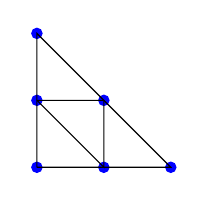
\begin{tikzpicture}[scale=1.7]

    \coordinate (0) at (0,0);
    \coordinate (1) at (1,0);
    \coordinate (2) at (0,1);

    \coordinate (3) at (0,0.5);
    \coordinate (4) at (0.5,0.5);
    \coordinate (5) at (0.5,0);

    \foreach \i in {0,1, 2, 3, 4, 5}
    \draw[blue,fill=blue] (\i) circle (1.1pt) node [below] {};


    \draw (0) --(1) -- (2) -- (0);
    \draw (3) --(4) -- (5) -- (3);

  \end{tikzpicture}
  \hfill\hfill
  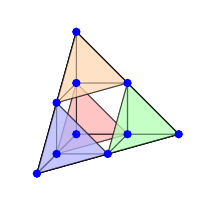
\begin{tikzpicture}[scale=1.3]

    \coordinate (0) at (0,0,0);
    \coordinate (1) at (0,0,1);
    \coordinate (2) at (1,0,0);
    \coordinate (3) at (0,1,0);
    \coordinate (4) at (0,0,0.5);
    \coordinate (6) at (0.5,0,0);
    \coordinate (7) at (0,0.5,0);
    \coordinate (5) at (0.5,0.0,0.5);
    \coordinate (8) at (0.0,0.5,0.5);
    \coordinate (9) at (0.5,0.5,0.0);

    \draw (0) -- (1) -- (2) -- (0);
    \draw (0) -- (1) -- (3) -- (0);
    \draw (1) -- (2) -- (3) -- (1);

    \draw[-, fill=red!30, opacity=.5] (4)--(6)--(7)--cycle;
    \draw[-, fill=red!30, opacity=.5] (0)--(6)--(7)--cycle;
    \draw[-, fill=red!30, opacity=.5] (0)--(4)--(7)--cycle;
    \draw[-, fill=red!30, opacity=.5] (0)--(4)--(6)--cycle;

    \draw[-, fill=blue!30, opacity=.5] (1)--(4)--(5)--cycle;
    \draw[-, fill=blue!30, opacity=.5] (1)--(4)--(8)--cycle;
    \draw[-, fill=blue!30, opacity=.5] (4)--(5)--(8)--cycle;
    \draw[-, fill=blue!30, opacity=.5] (1)--(5)--(8)--cycle;

    \draw[-, fill=green!30, opacity=.5] (2)--(5)--(6)--cycle;
    \draw[-, fill=green!30, opacity=.5] (2)--(6)--(9)--cycle;
    \draw[-, fill=green!30, opacity=.5] (2)--(5)--(9)--cycle;
    \draw[-, fill=green!30, opacity=.5] (5)--(6)--(9)--cycle;

    \draw[-, fill=orange!30, opacity=.5] (7)--(8)--(9)--cycle;
    \draw[-, fill=orange!30, opacity=.5] (3)--(7)--(9)--cycle;
    \draw[-, fill=orange!30, opacity=.5] (3)--(7)--(8)--cycle;
    \draw[-, fill=orange!30, opacity=.5] (3)--(8)--(9)--cycle;

    \foreach \i in {0,1,2,3,4,5,6,7,8,9}
    \draw[blue,fill=blue] (\i) circle (1.0pt) node [below] {};

  \end{tikzpicture}
  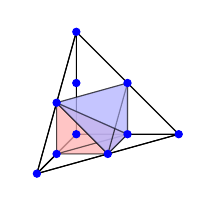
\begin{tikzpicture}[scale=1.3]

    \coordinate (0) at (0,0,0);
    \coordinate (1) at (0,0,1);
    \coordinate (2) at (1,0,0);
    \coordinate (3) at (0,1,0);
    \coordinate (4) at (0,0,0.5);
    \coordinate (6) at (0.5,0,0);
    \coordinate (7) at (0,0.5,0);
    \coordinate (5) at (0.5,0.0,0.5);
    \coordinate (8) at (0.0,0.5,0.5);
    \coordinate (9) at (0.5,0.5,0.0);

    \draw (0) -- (1) -- (2) -- (0);
    \draw (0) -- (1) -- (3) -- (0);
    \draw (1) -- (2) -- (3) -- (1);

    \draw[-, fill=red!30, opacity=.5] (4)--(5)--(6)--cycle;
    \draw[-, fill=red!30, opacity=.5] (4)--(5)--(8)--cycle;
    \draw[-, fill=red!30, opacity=.5] (4)--(6)--(8)--cycle;
    \draw[-, fill=red!30, opacity=.5] (5)--(6)--(8)--cycle;

%    \draw[-, fill=blue!30, opacity=.5] (4)--(6)--(7)--cycle;
%    \draw[-, fill=blue!30, opacity=.5] (4)--(6)--(8)--cycle;
%    \draw[-, fill=blue!30, opacity=.5] (4)--(7)--(8)--cycle;
%    \draw[-, fill=blue!30, opacity=.5] (6)--(7)--(8)--cycle;

%    \draw[-, fill=green!30, opacity=.5] (6)--(7)--(8)--cycle;
%    \draw[-, fill=green!30, opacity=.5] (6)--(7)--(9)--cycle;
%    \draw[-, fill=green!30, opacity=.5] (6)--(8)--(9)--cycle;
%    \draw[-, fill=green!30, opacity=.5] (7)--(8)--(9)--cycle;
%
    \draw[-, fill=blue!30, opacity=.5] (5)--(6)--(8)--cycle;
    \draw[-, fill=blue!30, opacity=.5] (5)--(6)--(9)--cycle;
    \draw[-, fill=blue!30, opacity=.5] (5)--(8)--(9)--cycle;
    \draw[-, fill=blue!30, opacity=.5] (6)--(8)--(9)--cycle;

    \foreach \i in {0,1,2,3,4,5,6,7,8,9}
    \draw[blue,fill=blue] (\i) circle (1.0pt) node [below] {};

  \end{tikzpicture}
  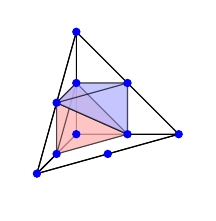
\begin{tikzpicture}[scale=1.3]

    \coordinate (0) at (0,0,0);
    \coordinate (1) at (0,0,1);
    \coordinate (2) at (1,0,0);
    \coordinate (3) at (0,1,0);
    \coordinate (4) at (0,0,0.5);
    \coordinate (6) at (0.5,0,0);
    \coordinate (7) at (0,0.5,0);
    \coordinate (5) at (0.5,0.0,0.5);
    \coordinate (8) at (0.0,0.5,0.5);
    \coordinate (9) at (0.5,0.5,0.0);

    \draw (0) -- (1) -- (2) -- (0);
    \draw (0) -- (1) -- (3) -- (0);
    \draw (1) -- (2) -- (3) -- (1);

%    \draw[-, fill=red!30, opacity=.5] (4)--(5)--(6)--cycle;
%    \draw[-, fill=red!30, opacity=.5] (4)--(5)--(8)--cycle;
%    \draw[-, fill=red!30, opacity=.5] (4)--(6)--(8)--cycle;
%    \draw[-, fill=red!30, opacity=.5] (5)--(6)--(8)--cycle;

    \draw[-, fill=red!30, opacity=.5] (4)--(6)--(7)--cycle;
    \draw[-, fill=red!30, opacity=.5] (4)--(6)--(8)--cycle;
    \draw[-, fill=red!30, opacity=.5] (4)--(7)--(8)--cycle;
    \draw[-, fill=red!30, opacity=.5] (6)--(7)--(8)--cycle;

    \draw[-, fill=blue!30, opacity=.5] (6)--(7)--(8)--cycle;
    \draw[-, fill=blue!30, opacity=.5] (6)--(7)--(9)--cycle;
    \draw[-, fill=blue!30, opacity=.5] (6)--(8)--(9)--cycle;
    \draw[-, fill=blue!30, opacity=.5] (7)--(8)--(9)--cycle;

%    \draw[-, fill=orange!30, opacity=.5] (5)--(6)--(8)--cycle;
%    \draw[-, fill=orange!30, opacity=.5] (5)--(6)--(9)--cycle;
%    \draw[-, fill=orange!30, opacity=.5] (5)--(8)--(9)--cycle;
%    \draw[-, fill=orange!30, opacity=.5] (6)--(8)--(9)--cycle;

    \foreach \i in {0,1,2,3,4,5,6,7,8,9}
    \draw[blue,fill=blue] (\i) circle (1.0pt) node [below] {};

  \end{tikzpicture}
  \hfill
  \phantom{.}

  % We definitely supported tri refinement in 9.3 - see 6ceb8b70559dc2274761a28dc7836f1e9602da8c (Dec 4, 2020)
  % and also 74b8171dd030a4b2de41955b8d913cde06974b91 (Feb 4, 2021)
  \caption{\it The previous release, 9.3 \cite{dealII93}, had
    added support for adaptive mesh 
  refinement with triangles. This release adds support for global
  tetrahedral refinement by subdividing each tetrahedron into eight
  children, as shown on the right.}
  \label{fig:refinement}
\end{figure}

\begin{itemize}
\item Experimental support for locally refined meshes: For finite
  element computations on locally refined
meshes, one needs (i) the possibility to locally refine the mesh (see
Figure~\ref{fig:refinement}), and (ii) appropriate hanging-node
constraints. Both are now available in 2D; for 3D, the implementation
of the constraint definitions is still in progress.
\item \texttt{QIteratedSimplex} allows to build composite simplex quadrature rules.
\item The new wrappers to the \texttt{CGAL} library allow to simply create simplex
meshes. For more details, see Section~\ref{sec:cgalwrappers}.
\end{itemize}

Furthermore, we have continued to remove uses of the
\texttt{GeometryInfo} class (which is specific to hypercube cells) from
the library, and to replace them by more general equivalent
functionality based on the
\texttt{ReferenceCell} class. Once all instances of
\texttt{GeometryInfo} are removed, we will deprecate the class.

%%%%%%%%%%%%%%%%%%%%%%%%%%%%%%%%%%%%%%%%%%%%%%%%%%%%%%%%%%%%%%%%%%%%%%%%%%%%%%%%
\subsection{Repartitioning of distributed meshes}\label{sec:repartitioning}

\dealii has two classes that support distributed storage of meshes:
\texttt{parallel::\allowbreak distributed::\allowbreak Triangulation}
(which in the following we will abbreviate as \texttt{p::d::T}) and
\texttt{parallel::\allowbreak fully\allowbreak distributed::\allowbreak
  Triangulation} (or, in short, \texttt{p::f::T}). The former is
partitioned based on the space-filling Morton (or Z-order) curve
implemented by the \pfrst backend. The latter, more recent
class is currently statically partitioned at creation time.

There are now new utility functions in the
\texttt{RepartitioningPolicyTools} namespace that can be
used to create a new \texttt{p::f::T} instance,
given a distributed triangulation (\texttt{p::f::T} or
\texttt{p::d::T}) and a vector that indicates the designated owner processes of locally
owned cells. This approach allows for partitioning \texttt{p::f::T}
based on arbitrary criteria. The workflow is shown in the following listing:
\begin{c++}
// original triangulation:
parallel::distributed::Triangulation<dim> tria(communicator);

// select a partitioning policy and use it:
const RepartitioningPolicyTools::CellWeightPolicy<dim> policy(tria, fu);
const auto construction_data = TriangulationDescription::Utilities::
  create_description_from_triangulation(tria, policy.partition(tria));

// create the new triangulation:
parallel::fullydistributed::Triangulation<dim> tria_pft(comm);
tria_pft.create_triangulation(construction_data);
\end{c++}

\begin{figure}
    \centering
    \def\svgwidth{0.8\columnwidth}
    \input{svg/repartitioning.pdf_tex}
    \caption{\it Visualization of the repartitioning process and the
      construction of the new mesh of process 0. Top
      left: Existing ownership of the cells of the mesh, distributed
      on four processes. Bottom left:
      Requested new ownership. Second column: Processes 0 and 1
      collect information about the cells they own or that are ghost
      cells. Processes 2 and 3 do not contribute to process 0. Third column: What
      processes 0 and 1 would send to process 0. Fourth column: The
      combined knowledge on process 0.}\label{fig:repartitioning}
\end{figure}

The setup process (of \texttt{construction\_data}) is visualized in Figure~\ref{fig:repartitioning}. At
first, locally owned cells and their
surrounding (ghost) cells are collected on each process and
sent to the new owner. On the
receiving site, the sets of all cells are combined and possible duplicates
are removed. This information is enough to construct a new triangulation.
For sending/receiving, we apply consensus-based algorithms~\cite{hoefler2010scalable}, which
we introduced into the library in release 9.2~\cite{dealII92} -- see
also Section~\ref{sec:CA}. This kind of consensus-based
algorithm is used also in \cite{ibanez2016pumi} for repartitioning.

In addition to the predefined partitioning policies, users
can write their own by implementing the
\texttt{RepartitioningPolicyTools::Base} interface. Like the
``active'' level of finest cells, the scheme also allows for
arbitrarily repartitioned multigrid levels.

In future releases, we plan to add support for repartitioning based on distributed graph
partitioning libraries, e.g., \texttt{ParMETIS} or \texttt{Zoltan}. Furthermore, we intend to extend
\texttt{p::f::T} to support adaptive mesh refinement, completing \texttt{p::f::T}
as a complement to \texttt{p::d::T}.



%%%%%%%%%%%%%%%%%%%%%%%%%%%%%%%%%%%%%%%%%%%%%%%%%%%%%%%%%%%%%%%%%%%%%%%%%%%%%%%%
\subsection{Advances in matrix-free infrastructure}\label{sec:mf}

The matrix-free infrastructure of \dealii is used to solve problems
without assembling matrices, providing only the action of the matrix
instead. It has seen a number of new features in this release, the most
notable ones being:
\begin{itemize}
\item Improved support for computations with Hessians of shape functions: just like values and gradients, Hessians can be
now evaluated and integrated during matrix-free loops
both for cells and faces. This could enable, for example, writing
a matrix-free version of step-47, which solves the biharmonic equation with the discontinuous Galerkin method.
\item Cell-centric loops now also allow access to gradients and Hessians
of neighboring cells on faces. The major difficulty here was the relative orientation
of cells on unstructured meshes.
\item Users can now create their own cell batches, by providing \texttt{FEEvaluation::reinit()} a list of cell IDs. \texttt{FEEvaluation}
accesses the appropriate data and reshuffles mapping data accordingly on
the fly in order to enable vectorization over cells. The new feature is useful in several
contexts. Examples are simulations with sharp interfaces (e.g., two-phase flow
or shock capturing), where one needs to treat cells that are ``cut'' by
the interface in a special way. A challenge is that cell batches
might contain cut or non-cut cells, making the vectorization of these operations potentially more complicated. Previous functionality has provided the option of masking certain cells in cell batches, which works well if
the code paths do not diverge too much. Another way is to
categorize cells during \texttt{MatrixFree::reinit()} in such a way that mixed cell batches do not occur. However, \texttt{MatrixFree::reinit()}
might be too expensive if recategorization needs to happen very frequently to follow the dynamics of a system, e.g., in each time step. Despite some overhead compared to static matrix-free loops, the new feature can be the best option in these scenarios.
\item Initial support for H(div)-conforming elements with Piola transform, based on Raviart--Thomas finite element spaces with the updated class \texttt{FE\_RaviartThomasNodal}, has been added. This feature is currently limited to meshes in standard orientation and affine geometries. Full support and performance optimizations will be provided in a future release.
\item Selected matrix-free algorithms can now exploit additional data locality
  between the matrix-vector product and vector operations happening nearby in
  an algorithm. Interfaces have been added to both the
  \texttt{PreconditionChebyshev} class (a frequently used smoother in multigrid
  methods) and the conjugate gradient implementation in \texttt{SolverCG}.
  From the user's perspective, an operator needs to define a \texttt{vmult} operation,
  taking two additional \texttt{std::function} arguments. The first function
  defines the operation to be scheduled on the vector entries before the
  matrix-vector product touches them, and the second what happens
  afterward. The new features also include a renumbering to maximize data
  locality. The theory is described in the
  contribution~\cite{kronbichler2022cg}.
\end{itemize}
Besides these new features, we improved the performance of
hanging-node-constraint evaluation on the CPU. Instead of performing
quasi-dense matrix-vector multiplications~\cite{KronbichlerKormann2012}, we now use an
approach based on in-place interpolation and sum factorization, similar
to what was already done in the GPU code~\cite{ljungkvist2017matrix}. In \cite{munch2022hn}, the algorithm is described
and performance numbers are shown, indicating a reduction
of overhead of cells with hanging nodes by a factor of ten.

Finally, we have performed a major restructuring of the internals
of the \texttt{FEEvaluation} classes. This reduces some overheads for low polynomial degrees and will enable us to add support for new element types in the future.

We would like to remind users that we transitioned from the use of Booleans
to flags to configure the evaluation and integration process of \texttt{FEEvaluation}
and \texttt{FEFaceEvaluation}:

\begin{c++}
fe_eval.evaluate(false, true, false)         // old (deprecated)
fe_eval.evaluate(EvaluationFlags::gradients) // new
\end{c++}

%\begin{c++}
%additional_data.mapping_update_flags = ... | update_hessians;
%\end{c++}
%
%\begin{c++}
%FEEvaluation<dim> phi(matrix_free);
%
%phi.reinit(cell);
%phi.gather_evaluate(src, ... | EvaluationFlags::hessians);
%
%for(const auto q : phi.quadrature_point_indices())
%  phi.submit_hessian(phi.get_hessian(q), q);
%
%phi.integrate_scatter(... | EvaluationFlags::hessians, dst);
%\end{c++}
%
%... similar for faces; can be used to implement biharmonic equation (like in
%step-X)


%%%%%%%%%%%%%%%%%%%%%%%%%%%%%%%%%%%%%%%%%%%%%%%%%%%%%%%%%%%%%%%%%%%%%%%%%%%%%%%%
\subsection{Advances in multigrid infrastructure}\label{sec:multigrid}

In release 9.3~\cite{dealII93}, we added support for global-coarsening multigrid in
addition to the established local-smoothing infrastructure. Global
coarsening algorithms smoothen over the whole computational domain on each
multigrid level, which is obtained by coarsening the finest cells of
the next finer multigrid level.
For this purpose, we use a sequence of triangulations, and we perform
the smoothing only on their active levels. To create the sequence of
triangulations, one can use the functions \texttt{MGTransferGlobalCoarseningTools::create\_geometric\_coarsening\_sequence()}. A new version takes an
instance of \texttt{RepartitioningPolicyTools::Base} (see Subsection~\ref{sec:repartitioning}) as argument, which allows specifying the parallel
distribution of each multigrid level (in contrast to the fixed first-child policy in the case of local smoothing). These features have been developed and tuned for running on a supercomputer scale
with complicated coarse meshes as presented in \cite{kronbichler2021next}.
Furthermore, we added support for block vectors,
fixed a number of limitations, and performed performance optimizations of
the transfer operator; particularly, the redundant copy from/to temporary vectors
has been eliminated. Furthermore, hanging-node constraints are applied
efficiently in the same way as in the matrix-free loops (see Subsection~\ref{sec:mf}).

In \cite{munch2022gc}, the performance of the local-smoothing and global-coarsening
infrastructure of \dealii was compared for locally refined meshes. The results indicate that
the local definition of multigrid levels might introduce load imbalances
in the case of local smoothing so that global coarsening is favorable despite
potentially more expensive intergrid transfers. In order to judge the benefits
of one approach against the other, \dealii provides new functions
\texttt{workload\_imbalance()} and \texttt{vertical\_communication\_efficiency()}
in the \texttt{MGTools} namespace for the  estimation of the imbalance during, e.g.,
smoothing or the
communication efficiency during intergrid transfer, purely based on the given mesh.
% MK: I would not add this part, it does not really fit into this paper as
% there is nothing to report at this point (and we should then add references
% to the actual literature).
%The publication \cite{munch2022gc} also points out that not
%all types of smoothers are applicable for global coarsening due to the
%presence of hanging nodes, which is a motivation to add new smoother types
%to \dealii in the future.

%%%%%%%%%%%%%%%%%%%%%%%%%%%%%%%%%%%%%%%%%%%%%%%%%%%%%%%%%%%%%%%%%%%%%%%%%%%%%%%%
\subsection{CutFEM support}\label{sec:cut}

Several classes have been added to the \texttt{NonMatching} namespace to enable the use of cut finite element methods~\cite{burman_cutfem_2015}.
In the literature, these types of methods are also referred to as immersed, extended, or fictitious finite element methods.
Here, the domain, $\Omega$, is immersed in the background mesh, as illustrated in Fig.~\ref{fig:immersed-domain}.
Often, one solves for the degrees of freedom of the smallest submesh
which completely covers the domain, i.e., the blue and yellow cells of
Fig.~\ref{fig:location-to-level-set}.
The bilinear form in the weak form would then, for example, look like
\begin{equation}
  a(u,v) = (\nabla u, \nabla v)_\Omega - (\partial_n u, v)_\Gamma + \ldots
\end{equation}
Thus, when assembling on a cut cell, we are
required to integrate over the part of the domain and the part of the boundary, $\Gamma = \partial \Omega$, that falls inside the cell:
$K\cap \Omega$ and $K \cap \Gamma$.
Many of the new classes that support these operations assume that the domain is described by a level set function,
$\psi : \mathbb{R}^d \to \mathbb{R}$, such that
\begin{align}\label{eq:levelset}
  \Omega = \{x \in \mathbb{R}^d : \psi(x)<0\},
  \qquad
  \Gamma = \{x \in \mathbb{R}^d : \psi(x) = 0\}.
\end{align}



\begin{figure}
  \centering
  \begin{subfigure}[b]{0.3\textwidth}
    \centering
    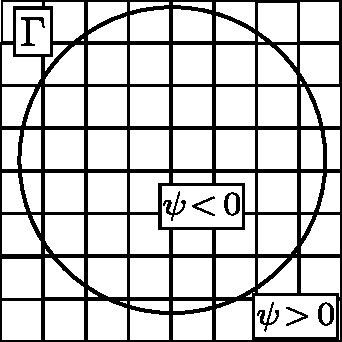
\includegraphics[height=.12\paperheight]{svg/immersed-domain.pdf}
    \caption{\label{fig:immersed-domain}}
  \end{subfigure}
  \qquad
  \begin{subfigure}[b]{0.3\textwidth}
    \centering
    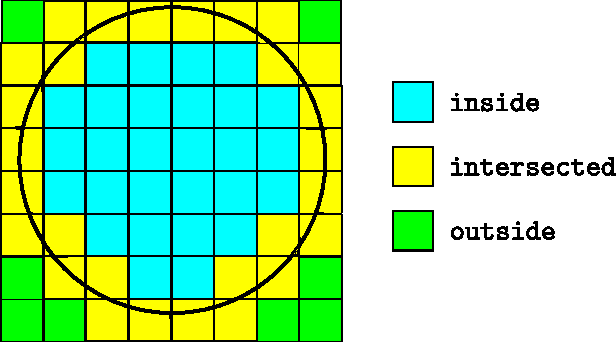
\includegraphics[height=.12\paperheight]{svg/location-to-level-set.pdf}
    \caption{ \label{fig:location-to-level-set}}
  \end{subfigure}
  \caption{\it (a) Domain immersed in a background mesh. (b) Value of \texttt{LocationToLevelSet} for each cell.}
%\end{figure}
%
%\begin{figure}
  \centering
  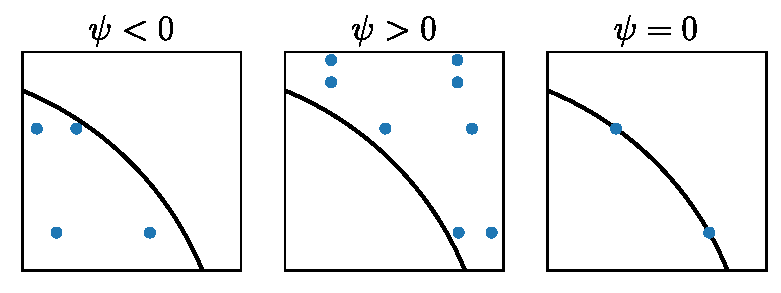
\includegraphics[width=.4\paperwidth]{svg/immersed_quadratures.pdf}
  \caption{\it Quadrature points for integrating over the three different regions of a cell cut by the zero contour of the level set function, $\psi$. \label{fig:immersed_quadratures}}
\end{figure}

Specifically, the following are the key new classes and functions:
\begin{itemize}
  \item The \texttt{MeshClassifier} class identifies how the active cells and faces are located relative to the zero contour of the level set function, as illustrated in Figure~\ref{fig:location-to-level-set}. Its member function \texttt{location\_to\_level\_set()} takes a cell or face and
        returns an enum, \texttt{LocationToLevelSet}, with values \{\texttt{inside}, \texttt{outside}, \texttt{intersected}\}.
        This information is typically needed when choosing what element a cell of the \texttt{DoFHandler} should use.

  \item The \texttt{QuadratureGenerator} class, which implements the algorithm in \cite{saye2015}, generates high-order quadrature rules for the three different regions of a \texttt{BoundingBox}, $B$, defined by the sign of the level set function:
        \begin{align}\label{eq:boundingbox}
          B \cap \Omega = \{ x\in B:  \psi(x) < 0 \},  \quad
          B \cap \Gamma = \{ x\in B:  \psi(x) = 0 \},  \quad
          \{ x\in B:  \psi(x) > 0 \}.
        \end{align}
        An example of these quadratures is shown in Figure~\ref{fig:immersed_quadratures}.
        The \texttt{FaceQuadratureGenerator} class does the same for faces.
        Furthermore, the new classes \texttt{DiscreteQuadratureGenerator} and \texttt{DiscreteFaceQuadratureGenerator} can be used to generate these quadrature rules over a cell or face when the level set function lies in a finite element space: $\psi_h \in V_h$, and when the reference cell of the cell or face is a hypercube.

  \item \texttt{ImmersedSurfaceQuadrature} is a class representing a quadrature rule over a $(d-1)$-dimensional surface embedded in $\mathbb{R}^d$ ($\psi = 0$ in Figure~\ref{fig:immersed_quadratures}). In addition to the weight, it stores the unit normal to the surface, for each quadrature point. This is needed to transform the quadrature rule from reference space to real space.

  \item \texttt{FEImmersedSurfaceValues} is an \texttt{FEFaceValues}-like class for evaluating real space values based on an \texttt{ImmersedSurfaceQuadrature}.

  \item \texttt{NonMatching::FEValues} combines the functionality of
    several of the above classes to simplify assembly of linear systems. It works similarly to \texttt{hp::FEValues}:
  When calling the \texttt{reinit()} function, immersed quadrature rules are generated in the background and
  \texttt{FEValues} objects for the inside/outside region and a \texttt{FEImmersedSurfaceValues} object for the surface regions are set up internally. These can then be obtained using getter-functions (\texttt{get\_inside/outside/surface\_fe\_values()}) and used for the assembly.
  Since the generation of immersed quadrature rules is not cheap,
  \texttt{NonMatching::FEValues} calls  \texttt{QuadratureGenerator} only if needed, i.e., if the cell is intersected. If not, already cached \texttt{FEValues} objects will be returned by the getter functions.
  Correspondingly, the class \texttt{NonMatching::FEInterfaceValues} generates
  \texttt{FEInterfaceValues} objects for assembling face terms over $F \cap \{x : \psi(x) < 0 \}$ or $F \cap \{x : \psi(x) > 0 \}$.
\end{itemize}
The new \texttt{step-85} tutorial illustrates how many of these classes work together.




%%%%%%%%%%%%%%%%%%%%%%%%%%%%%%%%%%%%%%%%%%%%%%%%%%%%%%%%%%%%%%%%%%%%%%%%%%%%%%%%
\subsection{Experimental integration of the Computational Geometry Algorithms
  Library (CGAL)}\label{sec:cgalwrappers}

The Computational Geometry Algorithms Library (CGAL, \url{https://www.cgal.org/}) is a widely used
library to describe geometries and meshes \cite{cgal}. \dealii now
has wrappers for CGAL classes and functions, provided in the new
namespace \texttt{CGALWrappers}, and implementing functionality
spanning from mesh generation to boolean operations between \dealii
triangulations and cells. These wrappers are enabled only if \dealii
is compiled with \texttt{C++17}. \textit{Note: This feature is still experimental and
interfaces might change during the next release cycle.}

The main mesh generation function is
\texttt{GridGenerator::implicit\_function()}, which creates a \texttt{Triangulation<dim,3>} out of the zero level set of an implicit function $\psi$ similar to \eqref{eq:levelset}.
For \texttt{dim==3}, the mesh consists of tetrahedra. A prototypical use case is the following, where the surface is the zero level set of Taubin's heart function $f=\bigl ( x^2 + \frac{9y^2}{4} +z^2 -1 \bigr ) -x^2 z^3 - \frac{9y^2z^3}{80}$. The resulting \texttt{Triangulation<3>} is shown in Figure~\ref{fig:heart_tria}
and the required steps are:
\begin{c++}
// 1) An implicit function, e.g., Taubin's heart surface (not shown)
ImplicitFunction implicit_fu;

// 2) configure output mesh (optional)
CGALWrappers::AdditionalData<3> data; data.cell_size = .05;

// 3) create mesh
Triangulation<3> tria;
GridGenerator::implicit_function(tria, implicit_fu, data, {0, 0, 0}, 10.0);
\end{c++}

A related function is
\texttt{GridGenerator::surface\_mesh\_to\_volumetric\_mesh()}, which
computes a tetrahedral volume triangulation \texttt{Triangulation<3>}, based on a
given surface triangulation \texttt{Triangulation<2,3>} that bounds
the three dimensional shape.

CGAL also provides Boolean operations on meshes, as available in the
utility function
\texttt{CGALWrappers::\allowbreak{}compute\_boolean\_operation()}. The
available operations are \textit{co-refinement}, \textit{intersection},
\textit{union}, and \textit{difference}. Oftentimes, boolean
operations and co-refinement around the intersection produces
badly shaped mesh cells. To overcome this issue, one can use \texttt{CGALWrappers::\allowbreak{}remesh\_surface()}. Figure~\ref{fig:corefinement_remeshed} shows a graphical example.
A possible workflow is the following:
\begin{c++}
// 1) create deal.II triangulations, e.g., cube and sphere (not shown)  
Triangulation<spacedim> tria0, tria1;

// 2) convert to CGAL surface meshes (assuming Kernel is already defined) 
CGAL::Surface_mesh<Kernel> surface_mesh0, surface_mesh1;
CGALWrappers::dealii_tria_to_cgal_surface_mesh(tria0, surface_mesh0);
CGALWrappers::dealii_tria_to_cgal_surface_mesh(tria1, surface_mesh1);

// 3) compute the union of the two meshes
CGALWrappers::compute_boolean_operation(surface_mesh0, surface_mesh1,
  BooleanOperation::compute_union, out_mesh);

// 4) convert CGAL surface mesh to deal.II surface mesh
Triangulation<2, 3> tria_out;
CGALWrappers::cgal_surface_mesh_to_dealii_triangulation(out_mesh, tria_out);

// 5) convert surface to volume mesh via surface_mesh_to_volumetric_mesh()
\end{c++}
The output of the boolean operation can be seen in Fig.~\ref{fig:corefinement}, while in Fig.~\ref{fig:corefinement_remeshed}
the same mesh has been remeshed.
\begin{figure}
  \centering
  \begin{subfigure}[b]{0.28\textwidth}
    \centering
    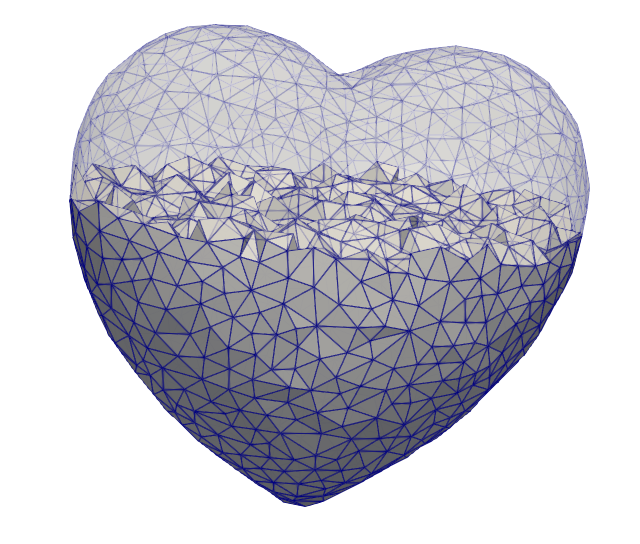
\includegraphics[width=\textwidth]{png/heart_implicit.png}
    \caption{\label{fig:heart_tria}}
  \end{subfigure}\qquad
  \hfill
  \begin{subfigure}[b]{0.28\textwidth}
    \centering
    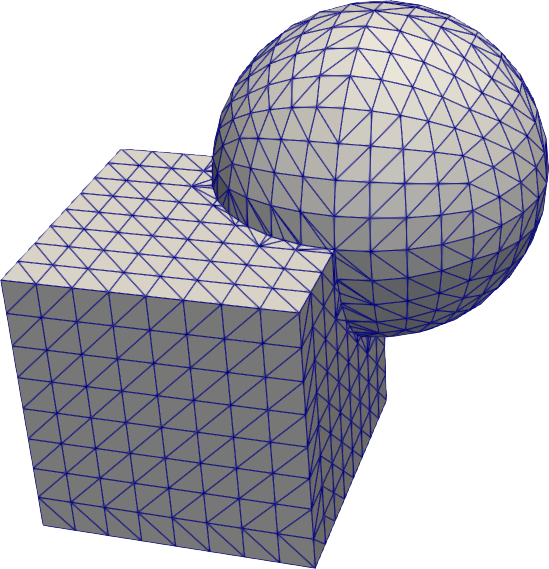
\includegraphics[width=\textwidth]{png/intersection_cube_sphere_mesh.png}
    \caption{\label{fig:corefinement}}
  \end{subfigure}
  \hfill
  \begin{subfigure}[b]{0.35\textwidth}
    \centering
    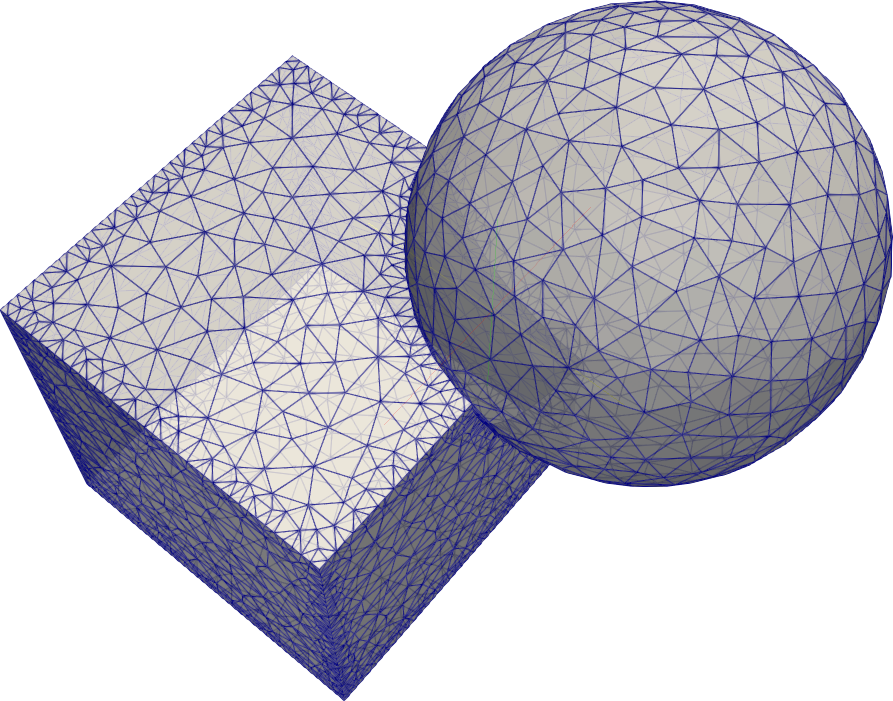
\includegraphics[width=\textwidth]{png/cube_sphere_remeshed.png}
    \caption{ \label{fig:corefinement_remeshed}}
  \end{subfigure}
  \caption{\it (a) Triangulation created by filling a heart-shaped surface implicitly described by a function $f$. (b) Union of a cube with a sphere with badly shaped cells at the intersection. (c) Remeshed version of the same triangulation.}
\end{figure}

\texttt{CGALWrappers::compute\_quadrature\_on\_boolean\_operation()} returns a \texttt{Quadrature<3>} that allows exact integration of polynomials on polyhedral elements coming out of a \texttt{BooleanOperation} between \dealii cells.
The quadrature rule is built by meshing the polyhedral region with tetrahedra, computing on each tetrahedron a \texttt{QGaussSimplex<3>} quadrature rule by using \texttt{QSimplex<3>::\allowbreak{}compute\_affine\_transformation()}, and finally
collecting all of the rules together, giving a \texttt{Quadrature<3>} formula on the \emph{physical} element.


These utility functions will be the building blocks for functions in the \texttt{NonMatching} namespace that will, e.g.,  assemble coupling terms like $(u,v)_{\Omega}$, with $\Omega$ a domain immersed in a fixed background mesh $B$ and $u,v$ finite element functions on $V_h(B)$, as needed, e.g., in 
the context of CutFEM (see Section~\ref{sec:cut}) or Nitsche's method to weakly impose boundary conditions at an interface. The same applies to coupling terms of the form $(u,q)_{\Omega}$ in formulations using Lagrange multipliers, where now $q \in Q_h(\Omega)$, with $Q_h(\Omega)$ the space of the multiplier variable.
Note that the most relevant difference between this and the \texttt{QuadratureGenerator} in Section~\ref{sec:cut} is that the \texttt{Quadrature} objects are created directly from two overlapping grids, one
spanning over $B$ and the other one over $\Omega$, and not from a level set function.



%%%%%%%%%%%%%%%%%%%%%%%%%%%%%%%%%%%%%%%%%%%%%%%%%%%%%%%%%%%%%%%%%%%%%%%%%%%%%%%%
\subsection{Performance improvement of particle infrastructure}\label{sec:particles}

In the release described herein, we have reorganized the data
structures and optimized the algorithms that support using particles
in \dealii. In our previously reported improvements~\citep{dealII93} we stored all particle data as a separate contiguous array for each particle property, but particle identifiers (IDs) were still stored in a multimap tree-like structure.

Our new particle containers are organized as follows: Particle IDs are stored in a list of dynamic arrays, each array containing the particle IDs of all particles in a unique cell. Each ID is a handle that determines the location of the data of this unique particle in the property arrays.
The list of ID arrays only contains entries for cells that contain particles. We keep a separate cache structure that contains pointers to the particular list entries for each cell. If a cell has no particles, this pointer is invalid.

This structure allows for the following significant performance improvements:

\begin{itemize}
\item All particle data (both their identifiers and their actual data) are now stored as separate and contiguous arrays in memory, which improves spatial locality for better prefetching of data and makes iterating over particles extremely efficient.
\item The choice of a list container that only includes entries for cells that contain particles means iteration is efficient, even if many cells in the domain do not contain any particles (as can be the case for discrete element methods~\cite{golshan2022lethe}).
\item Creating separate arrays for each cell allows us to easily move particle IDs from one cell to another as a local operation, affecting only the two cell containers in question. We take care to reuse allocated memory to minimize the number of memory reallocations.
\item The separate cache structure that contains entries for each cell allows quick random-access to the particles of a particular cell, and also allows to quickly determine if a particular cell has particles at all.
\end{itemize}

In addition to the new storage structure, we have made the following algorithmic improvements:
Determining if a particle is inside a cell after changing its position involves inverting the mapping for this cell. We have reorganized our algorithms to perform these inversions on a batch of particles in the same cell instead of particle-by-particle, which allows us to make use of vectorized instructions during the inversion using the generic scheme of~\cite{KronbichlerKormann2012}.
In addition, after sorting all particles into their new cells, the arrays that store particle properties are now sorted in the same order as the particle IDs in the list of arrays, which allows for cache efficient iteration over particle properties.
Because the particle IDs are already sorted in the intended order at this time, we can reorder the particle properties as part of a copy operation into a new data container that replaces the existing container. This approach avoids a costly in-place sort of the particle properties.

\begin{table}
  \caption{\it Timing of various particle operations for tutorial program \texttt{step-68} (particle advection in a 2D, Cartesian box) using 400,000 particles on a single process.}
  \label{tab:particle_timing}

  \centering
  \begin{tabular}{|c|c|c|c|}
    \hline
   Particle Operation & \dealii 9.3 & \dealii 9.4 & Speedup \\
   \hline
   Generation & 444 ms & 235 ms & 1.9$\times$ \\
   Iteration & 4.18 ms & 0.638 ms & 6.6$\times$ \\
   Advection & 37.8 ms & 33.9 ms & 1.15$\times$ \\
   Sorting & 21.9 ms & 9.27 ms & 2.4$\times$ \\
   \hline
  \end{tabular}
  \end{table}

We illustrate the combined effect of these performance improvements in Table~\ref{tab:particle_timing}. We measure the averaged compute time for four particle operations in a slightly modified version of the \dealii tutorial program \texttt{step-68} when advecting 400,000 particles on a single process (we have not observed any influence of the described changes on the parallel scalability of the algorithms).
The four operations we have measured are:
\begin{itemize}
\item Generation of a set of 400,000 particles at positions that are not aligned with the background mesh, i.e., the containing cell of each particle has to be identified with a search algorithm.
\item Iteration over the whole set of created particles, without
  significant computation and in particular without accessing particle data.
\item Advection of all particles, which involves iteration over all particles, evaluation of the finite element solution at the location of the particles, read and write access to the position of all particles to modify their location, and write access to the particle properties (to store their velocity for visualization purposes).
\item Sorting, i.e., the inversion of the mapping of each cell to find the new particle locations relative to this cell, and moving all particles that have left their original cell into new cells (both \dealii 9.3 and \dealii 9.4). In \dealii 9.4 this operation also includes reordering the particle properties for optimal iteration.
\end{itemize}

Table~\ref{tab:particle_timing} shows that all particle operations are
much faster in \dealii 9.4 than in version 9.3. In particular, operations that depend strongly on particle storage structure and require few fixed computations (like iteration and sorting) benefit massively from the above-mentioned optimizations. We note that the exact gains will depend strongly on the exact combination of geometry, mapping, dimensionality, and the number of particles per cell in any specific model, and can be smaller or larger than the measurements provided here.


%%%%%%%%%%%%%%%%%%%%%%%%%%%%%%%%%%%%%%%%%%%%%%%%%%%%%%%%%%%%%%%%%%%%%%%%%%%%%%%%
\subsection{Improvements to unstructured communication}
\label{sec:CA}

Many problems in parallel computations can be stated in the following
way: Each process in a parallel universe has a number of queries to
send to other processes that do not know that they will be asked, and
who will then have to respond with replies. This problem is solved by
``consensus algorithms''~\cite{hoefler2010scalable}. An example of where this problem appears is
given in Section~\ref{sec:repartitioning}.

\dealii has an implementation of these algorithms for some time,
but the current release substantially expands on it. Specifically, the
updated interfaces -- now based on function objects such as lambda
functions to formulate and process queries and replies -- can deal
with arbitrary data types for queries and replies, rather than only
arrays of data types natively supported by MPI. To make this possible,
the implementation packs and unpacks these objects into character
arrays via the \texttt{Utilities::pack()} and
\texttt{Utilities::unpack()} functions. We have also worked on making
these functions efficient: if the object to be packed is an array
(or array of arrays) of elements that satisfy the
\texttt{std::is\_trivially\_copyable} type trait, then the data is
copied into the character array via \texttt{std::memcpy}; only for
other objects do the packing and unpacking functions rely on BOOST's
serialization library.

A special case of consensus algorithms is where the sender does not
actually require an answer. This happens, for example, during repartitioning
of meshes (Section~\ref{sec:repartitioning}), where a process sends parts of
the new mesh to the new owners: the new owner does not know how many processes
will send it mesh parts and the sender only needs an acknowledgment that the
data has been received. Previously, such a case was implemented through a consensus
algorithm where the reply message is simply empty.
The rewritten interfaces now support this case more explicitly: Code using
these interfaces no longer has to provide functions that formulate
and read the (empty) replies, though internally these functions still
send around an empty reply; this case will be implemented in the
future, using the interfaces now already in place.

By the time of writing, \dealii uses consensus-based algorithms to determine
the owners of distributed index sets (\texttt{Utilities::MPI::Partitioner},
\texttt{Utilities::MPI::Noncontiguous\allowbreak Partitioner}, \texttt{internal::MatrixFreeFunctions::VectorDataExchange}; see~\cite{dealII91}),
to setup the global-coarsening transfer operators (see~\cite{dealII92} and
Section~\ref{sec:multigrid}), to repartition distributed meshes (see Section~\ref{sec:repartitioning}), and basis coupling algorithms between non-matching
meshes, based on the communication patters in \texttt{RemotePointeEvaluation} (see~\cite{dealII92}).

Finally, in the spirit of optimizing communication, the
\texttt{Utilities::MPI::broadcast()} function has been optimized for
objects that are arrays of data types natively supported by MPI and
which consequently can be sent without packing and unpacking.





%%%%%%%%%%%%%%%%%%%%%%%%%%%%%%%%%%%%%%%%%%%%%%%%%%%%%%%%%%%%%%%%%%%%%%%%%%%%%%%%
\subsection{New and improved tutorials and code gallery programs}
\label{subsec:steps}

Many of the \dealii tutorial programs were revised in a variety of ways
as part of this release. In addition, there are a number of new tutorial
programs:
\begin{itemize}
  \item
    \texttt{step-81} was contributed by Manaswinee Bezbaruah (Texas A\&M
    University) and Matthias Maier (Texas A\&M University). It explains how
    to solve the complex-valued time-harmonic Maxwell's equations for an
    optical scattering problem.
  \item
    \texttt{step-82} was contributed by Andrea Bonito (Texas A\&M
    University) and Diane Guignard (University of Ottawa). It shows how
    \dealii can be used to implement the local discontinuous Galerkin
    (LDG) method for approximating the solution to the bi-Laplacian
    problem. The method is an alternative to the C0IP method used in
    \texttt{step-47}.
  \item
    \texttt{step-85} was contributed by Simon Sticko (Uppsala University).
    It shows how to use the new CutFEM infrastructure to solve a Poisson
    problem on a circular domain that is embedded in a Cartesian background
    mesh.
\end{itemize}

There is also a new program in the code gallery (a collection of
user-contributed programs that often solve more complicated problems
than tutorial programs, and intended as starting points for further
research rather than as teaching tools):
\begin{itemize}
  \item ``TRBDF2-DG projection solver for the incompressible Navier--Stokes equations'' was contributed by Giuseppe Orlando (Politecnico di Milano). It shows
  how to solve the incompressible Navier--Stokes equations efficiently 
  with \dealii's matrix-free DG infrastructure, multigrid, and adaptive-mesh
  refinement. Interested readers are referred to~\cite{orlando2021efficient}.
\end{itemize}
Finally, the ``MCMC for the Laplace equation'' code gallery
program has been updated by providing MATLAB and Python versions of
the benchmark that is implemented in this code.



%%%%%%%%%%%%%%%%%%%%%%%%%%%%%%%%%%%%%%%%%%%%%%%%%%%%%%%%%%%%%%%%%%%%%%%%%%%%%%%%
\subsection{Incompatible changes}\label{subsec:deprecated}

The 9.4 release includes
\href{https://dealii.org/developer/doxygen/deal.II/changes_between_9_3_0_and_9_4_0.html}
{around 40 incompatible changes}; see \cite{changes94}. The majority of these changes
should not be visible to typical user codes; some remove previously
deprecated classes and functions; and the majority changes internal
interfaces that are not usually used in external
applications. That said, the following are worth mentioning since they
may have been more widely used:
\begin{itemize}
  \item In continuation of our attempt to merge the classes \texttt{DoFHandler} and \texttt{hp::DoFHandler}, we have removed the
  template parameter \texttt{DoFHandlerType} from a number of classes and
  functions, instead using \texttt{dim}/\texttt{spacedim} template arguments. Affected
  classes include \texttt{SolutionTransfer} and \texttt{DataOut}.
  \item \texttt{FE\_RaviartThomasNodal} now uses a different polynomial space to allow
  for a simpler use on faces in non-standard orientation. The new polynomials
  are anisotropic tensor products of Lagrange polynomials on the points of the
  Gauss--Lobatto quadrature formula. This change leads to different entries, for example, in
  the matrices and constraints, but no change in accuracy should be expected as
  the resulting basis spans the same polynomial space.
  \item The class \texttt{MappingQ} now applies a high-order mapping
    to all cells, not just the cells near the boundary, functionality
    that was previously provided by the \texttt{MappingQGeneric}
    class. The latter has been marked as deprecated.
  \item Changes to weighted repartitioning of
    \texttt{parallel::distributed::Triangulation} objects include
  the removal of the default weight of each cell in order to ensure
  consistency with the rest of the library and to improve flexibility.
\end{itemize}



%%%%%%%%%%%%%%%%%%%%%%%%%%%%%%%%%%%%%%%%%%%%%%%%%%%%%%%%%%%%%%%%%%%%%%%%%%%%%%%%
%%%%%%%%%%%%%%%%%%%%%%%%%%%%%%%%%%%%%%%%%%%%%%%%%%%%%%%%%%%%%%%%%%%%%%%%%%%%%%%%
%%%%%%%%%%%%%%%%%%%%%%%%%%%%%%%%%%%%%%%%%%%%%%%%%%%%%%%%%%%%%%%%%%%%%%%%%%%%%%%%
\section{How to cite \dealii}\label{sec:cite}

In order to justify the work the developers of \dealii put into this
software, we ask that papers using the library reference one of the
\dealii papers. This helps us justify the effort we put into this library.

There are various ways to reference \dealii. To acknowledge the use of
the current version of the library, \textbf{please reference the present
  document}. For up-to-date information and a bibtex entry
see
\begin{center}
  \url{https://www.dealii.org/publications.html}
\end{center}

The original \dealii paper containing an overview of its
architecture is \cite{BangerthHartmannKanschat2007}, and a more recent
publication documenting \dealii's design decisions is available as \cite{dealII2020design}. If you rely on
specific features of the library, please consider citing any of the
following:
\begin{multicols}{2}
  \vspace*{-36pt}
  \begin{itemize}[leftmargin=4mm]
    \item For geometric multigrid: \cite{Kanschat2004,JanssenKanschat2011,ClevengerHeisterKanschatKronbichler2019, munch2022gc};
    \item For distributed parallel computing: \cite{BangerthBursteddeHeisterKronbichler11};
    \item For $hp$-adaptivity: \cite{BangerthKayserHerold2007,fehling2022};
    \item For partition-of-unity (PUM) and finite element enrichment methods:
           \cite{Davydov2016};
    \item For matrix-free and fast assembly techniques:
          \cite{KronbichlerKormann2012,KronbichlerKormann2019};
    \item For computations on lower-dimensional manifolds:
          \cite{DeSimoneHeltaiManigrasso2009};
    \item For curved geometry representations and manifolds:
          \cite{HeltaiBangerthKronbichlerMola2019};
    \item For integration with CAD files and tools:
          \cite{HeltaiMola2015};
    \item For boundary element computations:
          \cite{GiulianiMolaHeltai-2018-a};
    \item For the \texttt{LinearOperator} and
      \texttt{Packaged\-Operation} facilities:
          \cite{MaierBardelloniHeltai-2016-a,MaierBardelloniHeltai-2016-b};
    \item For uses of the \texttt{WorkStream} interface:
          \cite{TKB16};
    \item For uses of the \texttt{ParameterAcceptor} concept, the
          \texttt{MeshWorker::ScratchData} base class, and the
          \texttt{ParsedConvergenceTable} class:
          \cite{SartoriGiulianiBardelloni-2018-a};
    \item For uses of the particle functionality in \dealii:
          \cite{GLHPB18}.
          \vfill\null
  \end{itemize}
\end{multicols}

\dealii can interface with many other libraries:
\begin{multicols}{3}
  \begin{itemize}[leftmargin=4mm]
    \item ADOL-C \cite{Griewank1996a,adol-c}
    \item ArborX \cite{lebrun2020arborx}
    \item ARPACK \cite{arpack}
    \item Assimp \cite{assimp}
    \item BLAS and LAPACK \cite{lapack}
    \item CGAL \cite{cgal}
    \item cuSOLVER \cite{cusolver}
    \item cuSPARSE \cite{cusparse}
    \item Gmsh \cite{geuzaine2009gmsh}
    \item GSL \cite{gsl2016}
    \item Ginkgo \cite{ginkgo-web-page}
    \item HDF5 \cite{hdf5}
    \item METIS \cite{karypis1998fast}
    \item MUMPS \cite{ADE00,MUMPS:1,MUMPS:2,mumps-web-page}
    \item muparser \cite{muparser-web-page}
    \item OpenCASCADE \cite{opencascade-web-page}
    \item p4est \cite{p4est,burstedde2020parallel}
    \item PETSc \cite{petsc-user-ref,petsc-web-page}
    \item ROL \cite{ridzal2014rapid}
    \item ScaLAPACK \cite{slug}
    \item SLEPc \cite{Hernandez:2005:SSF}
    \item SUNDIALS \cite{sundials}
    \item SymEngine \cite{symengine-web-page}
    \item TBB \cite{Rei07}
    \item Trilinos \cite{trilinos,trilinos-web-page}
    \item UMFPACK \cite{umfpack}
  \end{itemize}
\end{multicols}
Please consider citing the appropriate references if you use
interfaces to these libraries.

The two previous releases of \dealii can be cited as
\cite{dealII92,dealII93}.


\section{Acknowledgments}

\dealii is a world-wide project with dozens of contributors around the
globe. Other than the authors of this paper, the following people
contributed code to this release:\\
%
% Uwe Koecher doesn't usually show up in the changelog, but
% we should make sure he's listed.
%

% This is up-to-date as of 9.4 RC1 - should be the final list.
Pasquale      Africa,
Tyler         Anderson,
Francesco     Andreuzzi,
Mathias       Anselmann,
Maximilian    Bergbauer,
Manaswinee    Bezbaruah,
Bruno         Blais,
Till          Budde,
Fabian        Castelli,
Praveen       Chandrashekar,
Huimin        Chen,
Cu            Cui,
Ivo           Dravins,
Niklas        Fehn,
Corbin        Foucart,
Johannes      Friedlein,
Sebastian     Fuchs,
Daniel        Garcia-Sanchez,
Nicola        Giuliani,
Alexander     Grayver,
Diane         Guignard,
Jake          Harmon,
Sean          Ingimarson,
Pengfei       Jia,
Sebastian     Kinnewig,
Uwe           K{\"o}cher,
Katharina     Kormann,
Paras         Kumar,
Wenyu         Lei,
Alberto F.    Martin,
Nils          Much,
Lucas         Myers,
Justin        O'Connor,
Judith        Pauen,
Vachan        Potluri,
Raghunandan   Pratoori,
Sebastian     Proell,
Ce            Qin,
Reza          Rastak,
Jose E.       Roman,
Raphael       Schoof,
Magdalena     Schreter,
Konrad        Simon,
Daniel        Sun,
Kuljit S.     Virk,
Michał        Wichrowski,
Niklas        Wik,
Jiaqi         Zhang.


Their contributions are much appreciated!


\bigskip

\dealii and its developers are financially supported through a
variety of funding sources:


D.~Arndt and B.~Turcksin: Research sponsored by the Laboratory Directed Research and
Development Program of Oak Ridge National Laboratory, managed by UT-Battelle,
LLC, for the U. S. Department of Energy.

W.~Bangerth, T.~Heister, and R.~Gassm{\"o}ller were partially
supported by the Computational Infrastructure for Geodynamics initiative
(CIG), through the National Science Foundation (NSF) under Award
No.~EAR-1550901 and The University of California -- Davis.

W.~Bangerth and M.~Fehling were partially supported by Award OAC-1835673
as part of the Cyberinfrastructure for Sustained Scientific Innovation (CSSI)
program.

W.~Bangerth was also partially supported by Awards DMS-1821210 and EAR-1925595.

T.~Heister was also partially supported by NSF
Awards OAC-2015848, DMS-2028346, and
EAR-1925575, and by Technical Data Analysis, Inc. through US Navy STTR
Contract N68335-18-C-0011.

R.~Gassm{\"o}ller was also partially supported by the NSF Awards
EAR-1925677, and EAR-2054605.

L.~Heltai was partially supported by the Italian Ministry of Instruction,
University and Research (MIUR), under the 2017 PRIN project NA-FROM-PDEs MIUR
PE1, ``Numerical Analysis for Full and Reduced Order Methods for the efficient
and accurate solution of complex systems governed by Partial Differential
Equations''.

M.~Kronbichler and P.~Munch were partially supported by the
Bayerisches Kompetenznetzwerk
f\"ur Technisch-Wissen\-schaft\-li\-ches Hoch- und H\"ochstleistungsrechnen
(KONWIHR) in the context of the projects
``High-order matrix-free finite element implementations with
hybrid parallelization and improved data locality'' and ``Fast and scalable finite element algorithms for coupled multiphysics problems and non-matching grids''.

M.~Maier was partially supported by NSF Awards DMS-1912847 and DMS-2045636.

S.~Sticko was partially supported by eSSENCE of e-Science.

D.~Wells was supported by the NSF Award OAC-1931516.

The Interdisciplinary Center for Scientific Computing (IWR) at Heidelberg
University has provided hosting services for the \dealii web page.

\bibliography{paper}{}
\bibliographystyle{abbrv}

\end{document}
